\chapter{Overview of other used libraries} \label{chap:04}

This chapter contains a short description of the rest of the software, libraries and frameworks encountered during research. At the end of this chapter is mentioned PyNN, simulator-independent language for building neuronal network models \cite{davisonPyNNCommonInterface2009}. PyNN works as a frontend for Neuron, NEST and Brian simulators mentioned in the previous chapter.

\section{SNN toolbox}
SNN toolbox (SNN-TB) \cite{rueckauerConversionContinuousValuedDeep2017} is a conversion tool which automates the process of conversion of trained ANN to an SNN. The toolbox uses a deep learning model written in one of the supported ANN frameworks (Currently Keras / TensorFlow \cite{cholletKeras15}, Lasagne \cite{sanderdielemanLasagneFirst15}, Caffe \cite{jiaCaffeConvolutional14} and PyTorch \cite{paszkePyTorchImperative19}). The provided input model is parsed, and a general abstract model in Keras is derived. This internal model is used to achieve the actual conversion to the spiking network. That is achieved by replacing the analogue neurons to spiking integrate-and-fire neurons and altering the connection weights correspondingly. The resulting spiking model can be exported to several spiking simulators or deployed on dedicated neuromorphic chip-sets. Currently, the supported simulation platforms are PyNN, Brian2 and built-in MegaSim and INIsim simulators. Intel Loihi and SpiNNaker project are the supported hardware platforms at the moment. \Cref{fig:snn-tb_workflow} illustrates the workflow of the SNN toolbox.

\begin{figure}[htbp]
    \centering
    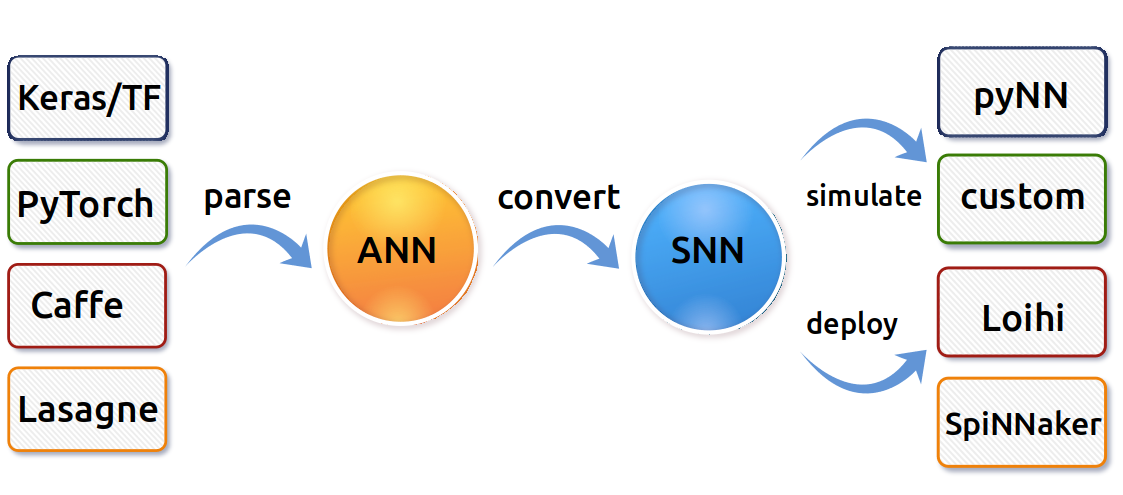
\includegraphics[width=\textwidth]{SNN-TB_workflow}
    \caption{The Illustration of the SNN toolbox workflow. An arbitrary supported deep learning model is transformed to an abstract Keras model, which is subsequently converted to a spiking network. Source: \url{https://snntoolbox.readthedocs.io/en/latest/guide/intro.html}}
    \label{fig:snn-tb_workflow}
\end{figure}

\section{Keras / TensorFlow}
Keras is a high-level deep learning API which can be used with multiple neural network or machine learning toolkits, mainly with TensorFlow. TensorFlow is an open-source machine learning platform. It consists of an interface for formulating machine learning algorithms and system-specific implementations to perform such algorithms.

\section{PyNN}
PyNN is a language for building models of neuronal networks independently of the used simulator. It provides a common API in the Python language to write the code and run it on multiple backends. PyNN API is designed to support neural networks models at a high-level of abstraction. Currently, Neuron, Brian (version 1) and NEST are supported simulators. PyNN also supports the SpiNNaker and BrainScaleS neuromorphic hardware and is partially compatible with NeuroML model description language. Figure in \cref{appendix:a} shows the architecture of the PyNN interface \cite{bruderleNeuroscientificModelingMixedSignal2009}.